\documentclass[10pt,a4paper]{article}

% ---------------------------------------------------------------------------
% Paquetes
% ---------------------------------------------------------------------------
\usepackage[utf8]{inputenc}
\usepackage[T1]{fontenc}
\usepackage[spanish,es-nodecimaldot]{babel}
\usepackage[a4paper,margin=2.5cm]{geometry}
\usepackage{graphicx}
\usepackage{float}
\usepackage{booktabs}
\usepackage{array}
\usepackage{amsmath}
\usepackage{listings}
\usepackage[hidelinks]{hyperref}

\lstset{
    basicstyle=\ttfamily\small,
    columns=fullflexible,
    frame=single,
    keepspaces=true,
    showstringspaces=false,
    breaklines=true
}

\graphicspath{
    {pics/}
    {../../TP2/top/informe/pics/}
}

% Marcas para resultados y figuras que se incorporarán en etapas posteriores.
\newcommand{\pendiente}[1]{\textit{[Completar: #1]}}
\newcommand{\figpendiente}[2]{%
    \begin{figure}[H]
        \centering
        \fbox{\parbox[c][4.2cm][c]{0.86\linewidth}{\centering #1}}
        \caption{#2}
    \end{figure}
}

% ---------------------------------------------------------------------------
% Documento
% ---------------------------------------------------------------------------
\begin{document}

\hypersetup{pageanchor=false}
\begin{titlepage}
\centering


\includegraphics[width=0.55\textwidth]{fulgor.png}

{\Huge\bfseries Trabajo Práctico N.\textsuperscript{o} 3\par}
\vspace{0.5cm}
{\LARGE Estimación y reducción de potencia en un remuestreador FIR\par}
\vspace{0.4cm}
{\large Inserción de ceros frente a descomposición polifásica\par}
\vspace{1.5cm}
{\Large Curso de Diseño Digital VLSI -- Fundación Fulgor\par}
\vfill

{\Large Damián Lugano\par}
\vspace{0.5cm}
{\large \today\par}

\end{titlepage}

\hypersetup{pageanchor=true}
\pagenumbering{roman}
\tableofcontents
\clearpage
\pagenumbering{arabic}

% ---------------------------------------------------------------------------
\section{Introducción}
\label{sec:introduccion}
% ---------------------------------------------------------------------------

\subsection{Objetivos}

El objetivo de este trabajo es implementar dos arquitecturas RTL de un mismo
remuestreador FIR de tasa $L/M=4/3$ y comparar su consumo de potencia. La primera
arquitectura inserta tres ceros entre muestras consecutivas y aplica un FIR de
64 taps, calculando únicamente las salidas que se conservan al diezmar por tres.
La segunda utiliza cuatro fases de 16 taps para calcular esas mismas salidas
directamente sobre las muestras originales.

En cada ciclo válido ambas arquitecturas reciben 90 muestras y producen un bloque
de 120 salidas, luego de su latencia de procesamiento. El FIR cumple las funciones
de anti-imagen después de la interpolación y anti-aliasing antes del diezmado.
El reloj trabaja a la tasa de bloques, $f_{\mathrm{clk}}=f_s/90$.

Ambas implementaciones deben producir exactamente la misma secuencia de salida.
Esta equivalencia funcional es una condición necesaria para que las diferencias
posteriores de potencia, área y timing puedan atribuirse a la arquitectura y no a
una diferencia en el procesamiento numérico.

Además de medir el consumo total, se busca comprender qué estructuras lo originan,
separar las componentes dinámica y estática, observar el efecto de los glitches y
evaluar técnicas de reducción de potencia sin perder equivalencia funcional ni
incumplir las restricciones de timing.

\subsection{Ejercicios solicitados}

El trabajo se organiza en los siguientes ejercicios:

\begin{enumerate}
    \item \textbf{Implementación, verificación y cierre de timing.} Desarrollar el
    modelo de punto fijo, verificar la equivalencia del remuestreo directo y
    polifásico sobre la secuencia completa y en bloques de 90 entradas, implementar
    ambas arquitecturas paralelas y determinar un período de trabajo común.

    \item \textbf{Anatomía del consumo.} Separar potencia de switching, potencia
    interna y leakage, e identificar los bloques que dominan el consumo.

    \item \textbf{Glitches.} Comparar la actividad espuria de las arquitecturas
    mediante simulaciones de compuertas con y sin retardos anotados.

    \item \textbf{Data gating.} Reducir la actividad de la arquitectura directa
    aislando los operandos durante los ciclos sin bloque válido. Comparar el
    forzado a cero con la retención del último bloque válido y estudiar la
    actividad de los multiplicadores asociados al relleno.

    \item \textbf{Clock gating.} Detener selectivamente el clock de registros que
    no necesitan actualizarse durante los ciclos sin bloque válido y cuantificar
    el ahorro para distintas fracciones de ciclos válidos.

    \item \textbf{Multi-$V_t$.} Evaluar el compromiso entre timing y leakage al
    utilizar celdas con distintas tensiones de umbral.

    \item \textbf{Arquitecturas opcionales.} Analizar el compromiso entre hardware
    compartido mediante plegado, paralelismo y aprovechamiento de la simetría
    de los coeficientes.
\end{enumerate}

% ---------------------------------------------------------------------------
\section{Marco teórico}
\label{sec:marco-teorico}
% ---------------------------------------------------------------------------


\subsection{Interpolación mediante inserción de ceros}

La interpolación digital permite incrementar la tasa de muestreo de una
señal discreta por un factor entero $L$. Para ello, se construye una
secuencia $x_u[n]$ intercalando $L-1$ ceros entre muestras consecutivas:

\begin{equation}
x_u[n]=
\begin{cases}
x[n/L], & n \equiv 0 \pmod L,\\
0,      & \text{en otro caso}.
\end{cases}
\label{eq:upsampling}
\end{equation}

La inserción de ceros aumenta la tasa de muestreo de $f_s$ a $Lf_s$,
pero también introduce imágenes espectrales. Para eliminarlas, se
aplica un filtro FIR pasabajos de $N$ coeficientes, cuya salida se
calcula mediante la convolución

\begin{equation}
y_u[n]=\sum_{k=0}^{N-1}h[k]x_u[n-k].
\label{eq:fir-directo}
\end{equation}

En una implementación directa, cada muestra de salida requiere
evaluar $N$ productos y acumular sus resultados. Sin embargo, cuando
$N$ es múltiplo de $L$, solamente $N/L$ posiciones de la ventana de
entrada corresponden a muestras originales. Las restantes $N-N/L$
posiciones contienen ceros insertados.

Por lo tanto, una proporción $(L-1)/L$ de los productos calculados
tiene resultado nulo. Esta redundancia motiva el uso de estructuras
polifásicas, que permiten reorganizar el filtrado y eliminar dichas
operaciones sin modificar la respuesta del sistema.

\subsection{Descomposición polifásica}

La descomposición polifásica consiste en separar el filtro prototipo
en $L$ subfiltros, agrupando los coeficientes según su posición
módulo $L$.

Considerando la ecuación~\eqref{eq:fir-directo}, se expresa el índice
de salida a tasa alta como $n=mL+p$, donde $p$ identifica la fase.
Debido a la inserción de ceros, únicamente contribuyen los términos
cuyos índices cumplen $k \equiv p \pmod L$.

Sustituyendo $k=rL+p$, se obtiene

\begin{equation}
y_u[mL+p]=
\sum_{r=0}^{N/L-1}h[rL+p]x[m-r].
\label{eq:polyphase}
\end{equation}

Se define entonces el conjunto de coeficientes correspondiente a
cada fase:

\begin{equation}
E_p[r]=h[rL+p],
\qquad p=0,\ldots,L-1.
\label{eq:phase-coefficients}
\end{equation}

De esta manera, el filtro original de $N$ coeficientes se reorganiza
en $L$ subfiltros de $N/L$ coeficientes cada uno.

Para los parámetros del trabajo, $L=4$ y $N=64$, se obtienen cuatro
fases de 16 coeficientes:

\begin{align}
E_0[r] &= h[4r], \nonumber\\
E_1[r] &= h[4r+1], \nonumber\\
E_2[r] &= h[4r+2], \nonumber\\
E_3[r] &= h[4r+3].
\label{eq:four-phases}
\end{align}

Cada salida requiere solamente 16 multiplicaciones, frente a las
64 de la implementación directa. La reducción aritmética teórica
es, por lo tanto, un factor $L=4$.

Esta transformación no modifica los coeficientes del filtro ni
su respuesta funcional. Únicamente reorganiza las operaciones
para evitar los productos asociados a las posiciones de relleno.

\subsection{Remuestreo racional y procesamiento paralelo}

El sistema implementado realiza un remuestreo racional por un factor
$L/M=4/3$. Para ello, después de la interpolación y el filtrado se
aplica un diezmado por $M=3$, conservando una de cada tres muestras
de la secuencia a tasa alta. El filtro debe eliminar las imágenes de la
interpolación y limitar el espectro antes del diezmado. Para cumplir ambas
funciones se utiliza un corte de $\pi/\max(L,M)=\pi/4$, referido a la tasa
alta $Lf_s$.

La salida del remuestreador directo queda definida por

\begin{equation}
y[n]=y_u[Mn]
=\sum_{k=0}^{N-1}h[k]x_u[Mn-k].
\label{eq:rational-direct}
\end{equation}

La formulación polifásica equivalente se obtiene definiendo

\begin{equation}
m_n=\left\lfloor\frac{Mn}{L}\right\rfloor,
\qquad
p_n=Mn\bmod L.
\label{eq:phase-selection}
\end{equation}

Así, cada muestra de salida puede calcularse directamente a
partir de la secuencia original:

\begin{equation}
y[n]=
\sum_{r=0}^{N/L-1}E_{p_n}[r]x[m_n-r].
\label{eq:rational-polyphase}
\end{equation}

Para $L=4$ y $M=3$, el patrón de fases es periódico:

\begin{equation}
p_n=3n\bmod4
\quad\Rightarrow\quad
\{0,3,2,1,0,3,2,1,\ldots\}.
\label{eq:phase-pattern}
\end{equation}

A diferencia de una implementación secuencial, donde las salidas
se producen individualmente, las arquitecturas de este trabajo
procesan bloques completos en paralelo.

En cada ciclo válido se reciben $P_{\mathrm{in}}=90$ muestras y
se calculan $P_{\mathrm{out}}=120$ salidas, cumpliendo

\begin{equation}
P_{\mathrm{out}}=
P_{\mathrm{in}}\frac{L}{M}=120.
\label{eq:parallelism}
\end{equation}

La tasa de muestras de entrada es $f_s=90f_{\mathrm{clk}}$ y la de salida es
$f_{\mathrm{out}}=120f_{\mathrm{clk}}=(4/3)f_s$ para bloques válidos en todos
los ciclos.

Para el bloque $b$ y la salida local $j$, con
$j=0,\ldots,119$, la selección polifásica está determinada por

\begin{equation}
m=90b+\left\lfloor\frac{3j}{4}\right\rfloor,
\qquad
p=3j\bmod4.
\label{eq:block-indexing}
\end{equation}

Como cada bloque contiene 30 períodos de tres entradas y cuatro
salidas, el patrón de fases se repite entre bloques. Por ello,
la selección de fase y los índices de muestras pueden determinarse
en tiempo de elaboración, sin necesidad de un contador de fase
dinámico.

Ambas arquitecturas requieren conservar información del bloque
anterior para mantener la continuidad del filtrado. La versión
directa almacena las últimas $N-1=63$ posiciones de tasa alta,
mientras que la versión polifásica conserva las últimas
$N/L-1=15$ muestras originales.

En la arquitectura directa se calculan las 120 salidas conservadas
por el diezmado, utilizando un FIR de 64 taps para cada una.
La versión polifásica calcula las mismas 120 salidas, pero emplea
un FIR de 16 taps con la fase correspondiente.

En consecuencia, las cantidades de multiplicadores son

\begin{equation}
N_{\mathrm{mult,directa}}=120\cdot64=7680,
\label{eq:mult-direct}
\end{equation}

\begin{equation}
N_{\mathrm{mult,poli}}=120\cdot16=1920.
\label{eq:mult-poly}
\end{equation}

Por construcción, 5760 multiplicadores de la arquitectura directa
procesan posiciones de relleno. Para evitar que la síntesis los
elimine por propagación de constantes, dichas posiciones se
alimentan mediante una entrada configurable \texttt{i\_fill},
cuyo valor se establece en cero durante la verificación.

\subsection{Componentes de la potencia}

La potencia total de un circuito CMOS se separa en

\begin{equation}
P_{\mathrm{total}}=P_{\mathrm{switching}}+P_{\mathrm{internal}}+P_{\mathrm{leakage}}.
\label{eq:power-components}
\end{equation}

La potencia de switching corresponde a la energía necesaria para cargar y descargar
las capacidades de las interconexiones y entradas de las celdas. Una aproximación
habitual es

\begin{equation}
P_{\mathrm{switching}}=\alpha C_L V_{DD}^{2}f_{\mathrm{clk}},
\label{eq:switching-power}
\end{equation}

donde $\alpha$ representa la actividad de conmutación. La potencia interna se
disipa dentro de las celdas debido a la carga de nodos internos y a la conducción
simultánea de transistores durante las transiciones. Ambas forman la potencia
dinámica y dependen de la actividad, la frecuencia, los slews y las cargas. Luego,
la potencia de leakage está presente incluso cuando el circuito no conmuta. Depende
del tipo de celda, su estado lógico, la tensión de alimentación y la temperatura, y
crece con el área implementada.

Para comparar arquitecturas que implementan el mismo remuestreador
se utiliza también la energía consumida por muestra de salida.
Considerando una tasa de salida $f_{\mathrm{out}}=(L/M)f_s$,

\begin{equation}
E_{\mathrm{muestra}}=
\frac{P_{\mathrm{total}}}{f_{\mathrm{out}}}
=
\frac{P_{\mathrm{total}}}{(L/M)f_s}.
\label{eq:energy-per-sample}
\end{equation}

Dado que ambas arquitecturas entregan $P_{\mathrm{out}}=120$
muestras por ciclo válido, para un procesamiento continuo se obtiene

\begin{equation}
E_{\mathrm{muestra}}=
\frac{P_{\mathrm{total}}}{120f_{\mathrm{clk}}}.
\label{eq:energy-per-sample-parallel}
\end{equation}

Si solamente una fracción $d$ de los ciclos contiene bloques válidos, la tasa
media de salidas útiles es $120d f_{\mathrm{clk}}$. En ese caso, la energía se
calcula como $E_{\mathrm{muestra}}=P_{\mathrm{total}}/(120d f_{\mathrm{clk}})$,
para contabilizar únicamente las muestras efectivamente entregadas.

\subsection{Glitches y actividad real}

Los glitches son transiciones espurias producidas cuando señales que convergen en
una compuerta llegan con retardos diferentes. Son frecuentes en multiplicadores y
árboles de sumadores, donde existen numerosos caminos combinacionales de distinta
profundidad. Para que un glitch aparezca deben existir convergencia de señales,
desbalance de tiempos de llegada, sensibilización lógica y un pulso suficientemente
largo para superar el filtrado inercial.

Una simulación RTL sin retardos no permite observar este fenómeno. Por ese motivo,
las estimaciones de potencia principales se realizarán con actividad obtenida de una
simulación de compuertas con SDF. El estímulo utilizado también resulta determinante:
comparar arquitecturas exige aplicar la misma secuencia y el mismo período de clock.

% ---------------------------------------------------------------------------
\section{Ejercicio 1: implementación, verificación y cierre de timing}
\label{sec:ejercicio-1}
% ---------------------------------------------------------------------------

El objetivo del primer ejercicio es implementar las dos arquitecturas, demostrar
que son funcionalmente equivalentes y preparar el flujo para determinar el período
mínimo, realizar GLS y obtener la primera estimación de potencia.

\subsection{Parámetros comunes}

La Tabla~\ref{tab:parametros-comunes} resume los parámetros empleados por las dos
arquitecturas.

\begin{table}[H]
    \centering
    \caption{Parámetros comunes del remuestreador $4/3$.}
    \label{tab:parametros-comunes}
    \begin{tabular}{@{}ll@{}}
        \toprule
        \textbf{Parámetro} & \textbf{Valor} \\
        \midrule
        Factor de interpolación, $L$ & 4 \\
        Factor de diezmado, $M$ & 3 \\
        Cantidad de taps del prototipo, $N$ & 64 \\
        Fases y taps por fase & 4 fases de 16 taps \\
        Paralelismo de entrada, $P_{\mathrm{in}}$ & 90 muestras/ciclo válido \\
        Paralelismo de salida, $P_{\mathrm{out}}$ & 120 muestras/ciclo válido \\
        Formato de entrada & signed Q1.11, 12 bits \\
        Formato de coeficientes & signed Q1.11, 12 bits \\
        Formato de salida & signed Q1.11, 12 bits \\
        Cantidad de bloques del estímulo & 23 \\
        Cantidad de muestras de entrada & 2070 \\
        Cantidad de muestras de salida & 2760, sin cola del FIR \\
        Tasa de salida & $(4/3)f_s$ \\
        Tasa del clock & $f_s/90$ \\
        Conversión a la salida & Truncamiento y saturación signed \\
        \bottomrule
    \end{tabular}
\end{table}

\subsection{Modelo de referencia en Python}
\label{sec:modelo-referencia}

\subsubsection*{Diseño y cuantización del filtro}

El filtro prototipo de 64 taps se diseñó mediante \texttt{firwin}, con una
ventana de Hamming y una frecuencia de corte normalizada a Nyquist de la tasa
alta igual a $1/\max(L,M)=1/4$. Es un pasabajos de fase lineal que cumple las
funciones de anti-imagen y anti-aliasing. Su ganancia se multiplicó por $L=4$
para compensar la pérdida de amplitud debida a la inserción de ceros. Luego se
redondearon los coeficientes al formato signed Q1.11.

La Tabla~\ref{tab:coeficientes-fases} contiene los 64 coeficientes enteros,
repartidos según $E_p[r]=h[4r+p]$. El coeficiente $E_p[0]$ multiplica la muestra
más reciente de la ventana.

\begin{table}[H]
    \centering
    \caption{Coeficientes enteros Q1.11. Los valores reales se obtienen al dividir
    las palabras de la tabla por $2^{11}$.}
    \label{tab:coeficientes-fases}
    \begin{tabular}{@{}rrrrr@{}}
        \toprule
        $r$ & $E_0[r]$ & $E_1[r]$ & $E_2[r]$ & $E_3[r]$ \\
        \midrule
        0 & -3 & -7 & -7 & -4 \\
        1 & 4 & 12 & 15 & 8 \\
        2 & -9 & -27 & -33 & -16 \\
        3 & 19 & 54 & 63 & 31 \\
        4 & -36 & -99 & -115 & -55 \\
        5 & 63 & 177 & 205 & 99 \\
        6 & -117 & -337 & -409 & -212 \\
        7 & 278 & 952 & 1601 & 1998 \\
        8 & 1998 & 1601 & 952 & 278 \\
        9 & -212 & -409 & -337 & -117 \\
        10 & 99 & 205 & 177 & 63 \\
        11 & -55 & -115 & -99 & -36 \\
        12 & 31 & 63 & 54 & 19 \\
        13 & -16 & -33 & -27 & -9 \\
        14 & 8 & 15 & 12 & 4 \\
        15 & -4 & -7 & -7 & -3 \\
        \bottomrule
    \end{tabular}
\end{table}

\begin{figure}[H]
    \centering
    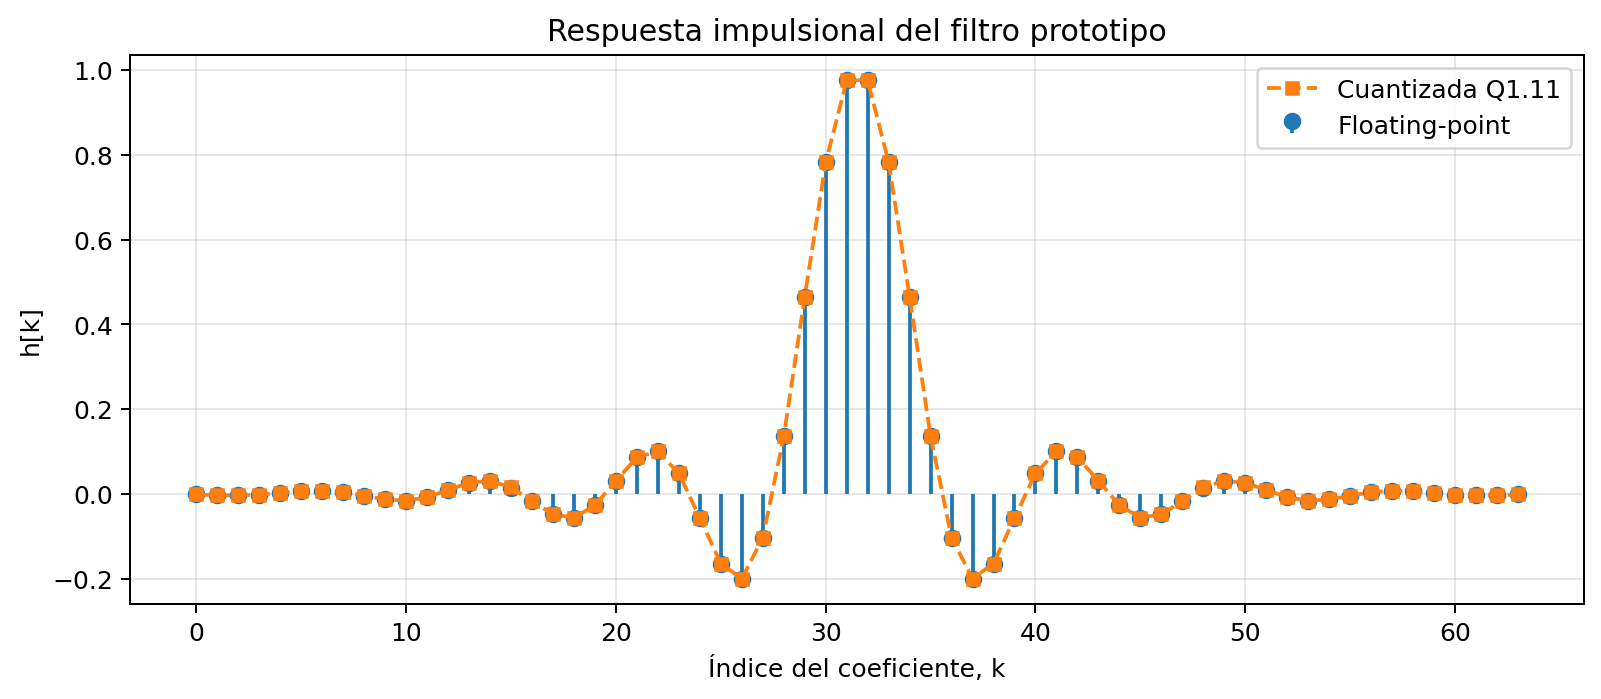
\includegraphics[width=0.88\linewidth]{filter_impulse_response.png}
    \caption{Respuesta impulsional del filtro prototipo antes y después de la
    cuantización.}
    \label{fig:filter-impulse-response}
\end{figure}

\begin{figure}[H]
    \centering
    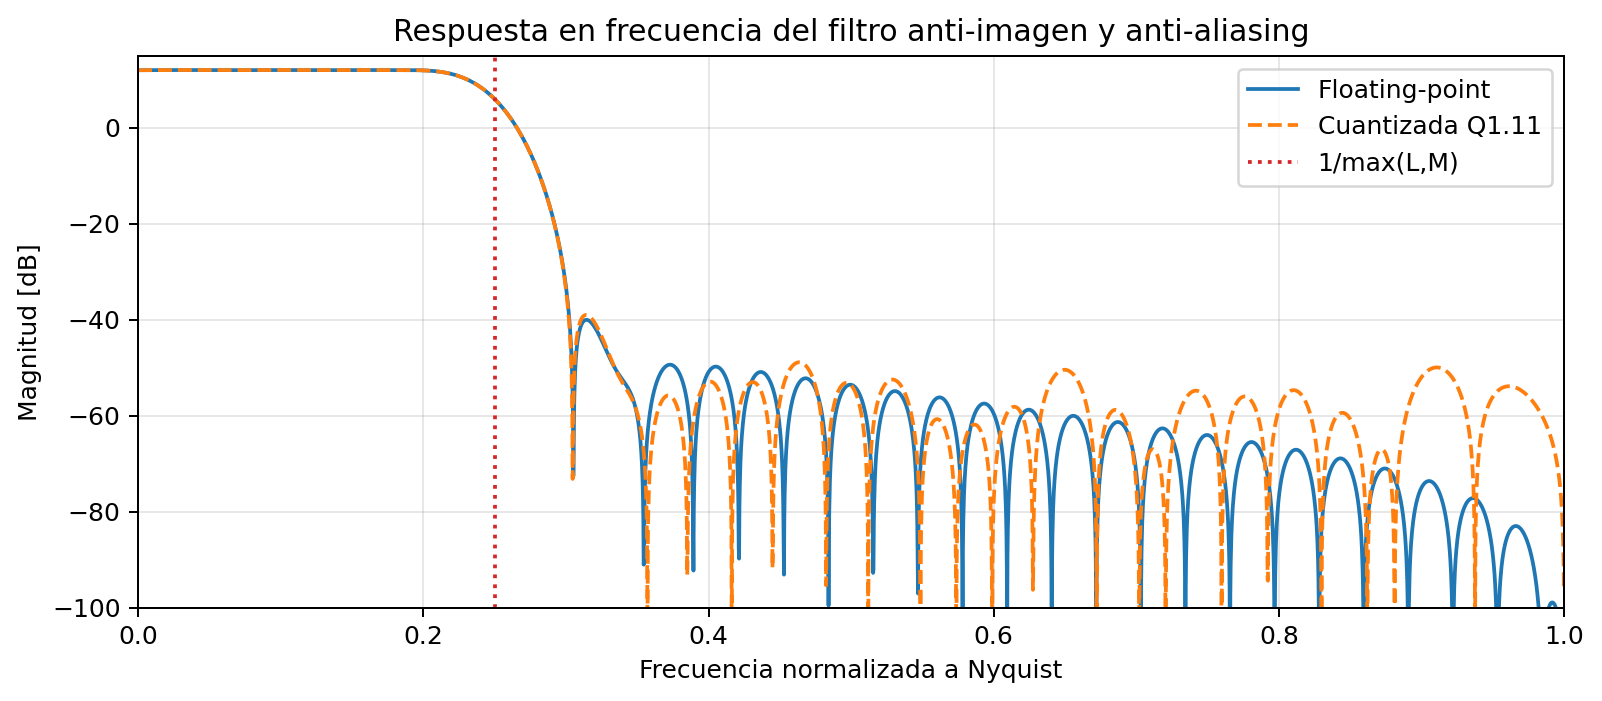
\includegraphics[width=0.88\linewidth]{filter_frequency_response.png}
    \caption{Respuesta en frecuencia del filtro pasabajos anti-imagen y anti-aliasing.}
    \label{fig:filter-frequency-response}
\end{figure}

\subsubsection*{Aritmética de punto fijo}

Las muestras y los coeficientes se representan con 12 bits y 11 bits
fraccionarios. Cada multiplicación genera un producto signed de 24 bits con 22
bits fraccionarios. Los productos alimentan un árbol balanceado de sumas sin
recortes intermedios. La clase \texttt{FixedPoint} aumenta automáticamente el
ancho en un bit por nivel: seis niveles para 64 productos y cuatro niveles
para 16 productos.

\begin{table}[H]
    \centering
    \caption{Formatos del modelo de referencia que debe respetar el RTL.}
    \label{tab:formatos-internos}
    \begin{tabular}{@{}lcc@{}}
        \toprule
        \textbf{Magnitud} & \textbf{Bits totales} & \textbf{Bits fraccionarios} \\
        \midrule
        Entrada y coeficiente & 12 & 11 \\
        Producto & 24 & 22 \\
        Acumulador directo, 64 taps & 30 & 22 \\
        Acumulador por fase, 16 taps & 28 & 22 \\
        Salida & 12 & 11 \\
        \bottomrule
    \end{tabular}
\end{table}

La conversión a la salida trunca los bits fraccionarios menos significativos y
satura cuando el resultado excede el rango signed de 12 bits. Para el truncado,
se descartan 11 bits mediante desplazamiento aritmético y luego se limita el 
entero al intervalo $[-2048,2047]$. Para valores negativos, este descarte 
corresponde a redondear hacia menos infinito. El truncamiento de la salida 
es independiente del redondeo utilizado al cuantizar los coeficientes y 
el estímulo.

\subsubsection*{Organización del modelo}

El archivo \path{TP3/model/reference_model.py} contiene un único bloque
aritmético, \texttt{fir\_model}. Esta función recibe una ventana de muestras y
un banco de coeficientes, y calcula una salida con la aritmética de la
Tabla~\ref{tab:formatos-internos}. El índice cero de la ventana corresponde
a la muestra más reciente.

La función \texttt{interp\_zeros} arma el regresor con las muestras de tasa
alta y las 63 posiciones de historia. Para la salida $n$ selecciona una ventana
que termina en la posición $3n$ del bloque actual y llama al FIR de 64 taps.
Únicamente calcula las salidas conservadas por el diezmado.

La función \texttt{interp\_poly} arma el regresor con las entradas originales
y las 15 muestras de historia. Para cada salida calcula $m=\lfloor3n/4\rfloor$
y $p=3n\bmod4$, toma la ventana que termina en la muestra $m$ y llama al mismo
FIR con los 16 coeficientes de la fase $p$.

Ambas funciones devuelven las salidas y la historia necesaria para la próxima
llamada. Cuando no se entrega historia, la memoria se inicializa en cero. Así,
las mismas funciones permiten procesar la secuencia completa o bloques de 90
entradas. El notebook \path{TP3/model/reference_model.ipynb} ejecuta las 
verificaciones, genera las figuras y exporta los vectores.

\subsubsection*{Estímulo de entrada común}

El estímulo está compuesto por dos tonos, ruido blanco de baja amplitud y una
normalización del pico a $-6\,\mathrm{dBFS}$:

\begin{equation}
x[n]=\sin(2\pi\,0.073n)
    +0.63\sin(2\pi\,0.181n+0.37)
    +0.04w[n].
\label{eq:stimulus}
\end{equation}

Se generan 2070 muestras, correspondientes a 23 bloques de 90 entradas.
La señal de la Ecuación~\eqref{eq:stimulus} se escala por un único factor para
fijar su pico en $-6\,\mathrm{dBFS}$. Se utiliza el generador
\texttt{default\_rng} y luego se cuantiza a Q1.11. De esta manera 
el estímulo es reproducible y puede reutilizarse sin modificaciones
en las simulaciones RTL, GLS y en todas las estimaciones de potencia.

\begin{figure}[H]
    \centering
    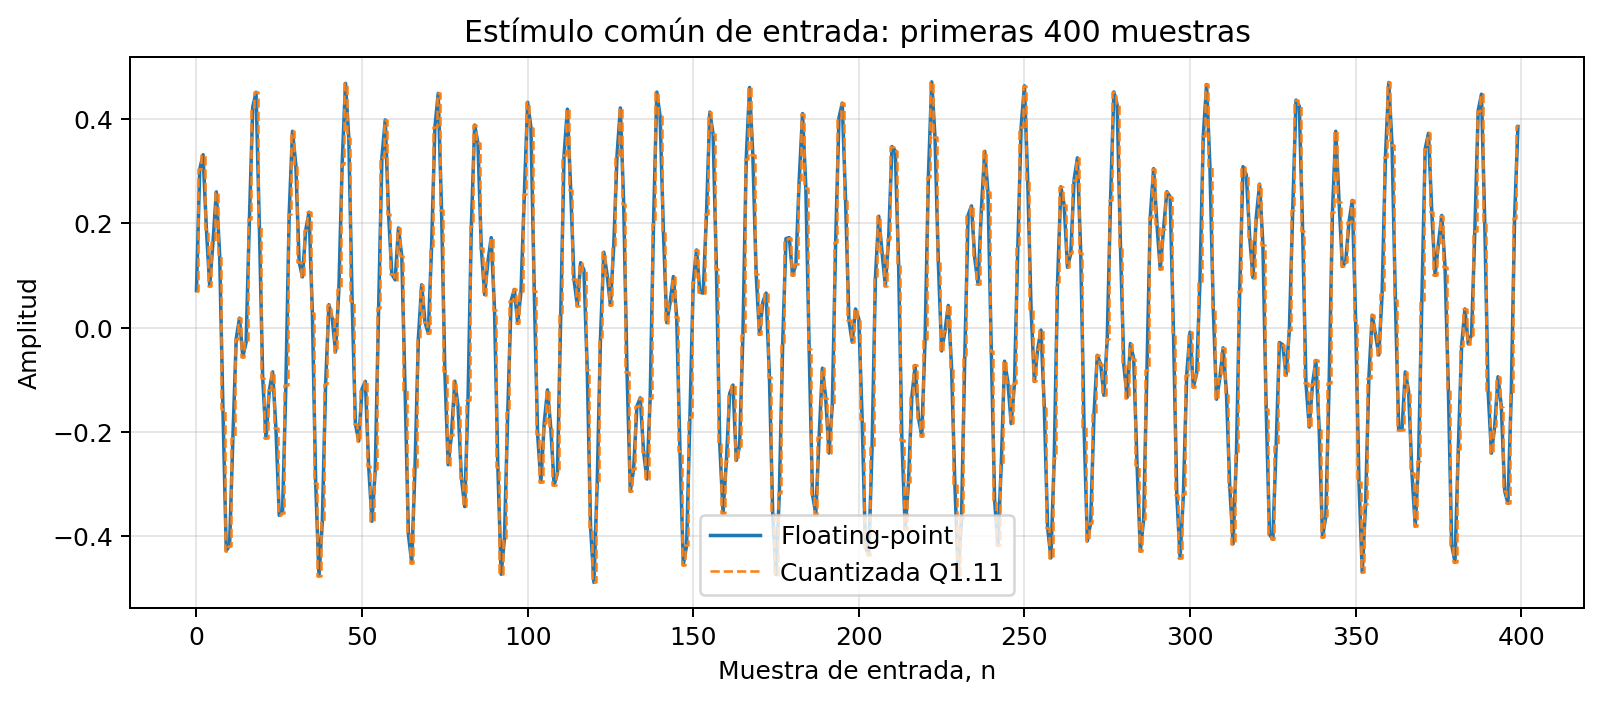
\includegraphics[width=0.88\linewidth]{input_signal.png}
    \caption{Señal de entrada utilizada como estímulo común.}
    \label{fig:input-signal}
\end{figure}

\begin{figure}[H]
    \centering
    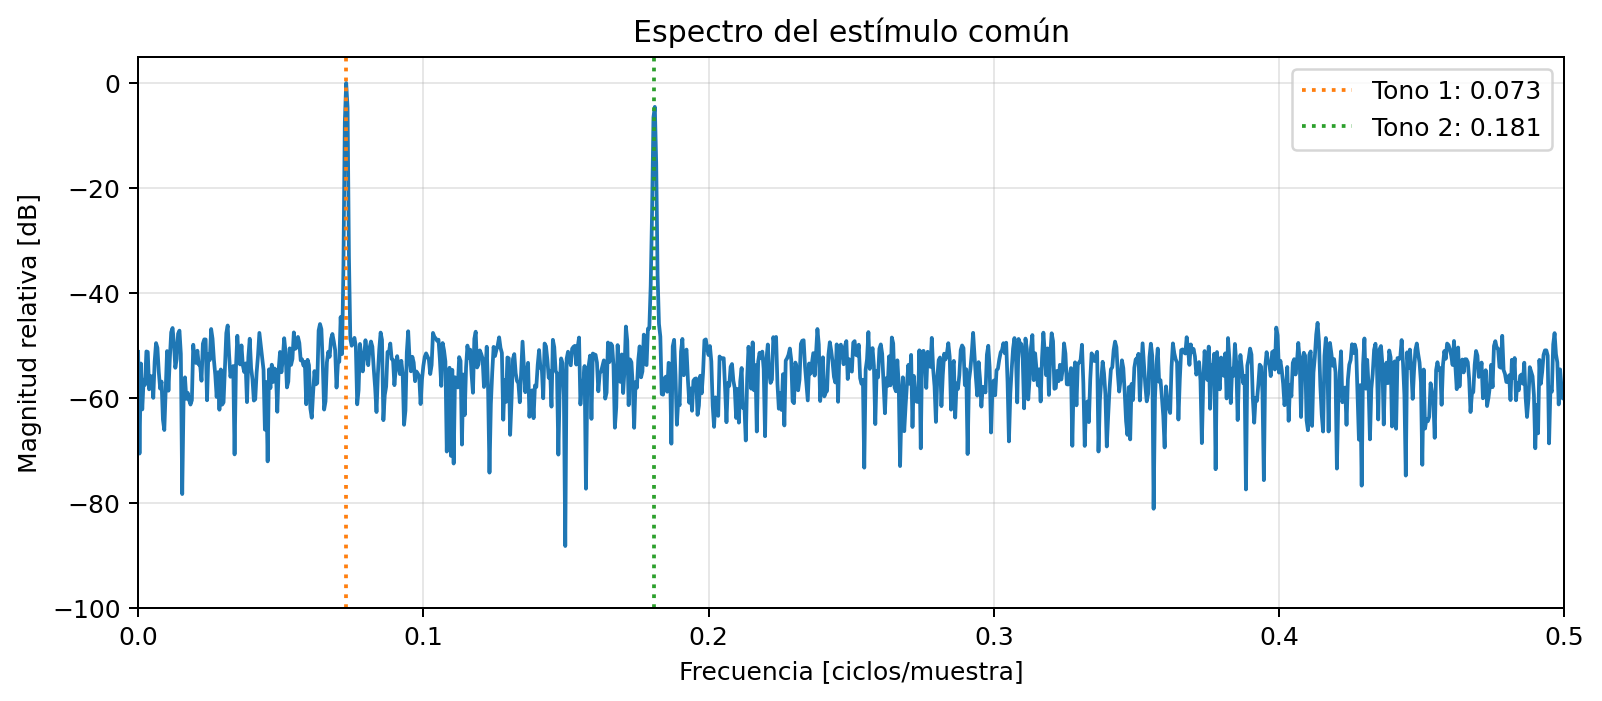
\includegraphics[width=0.88\linewidth]{input_spectrum.png}
    \caption{Espectro del estímulo común.}
    \label{fig:input-spectrum}
\end{figure}

\begin{figure}[H]
    \centering
    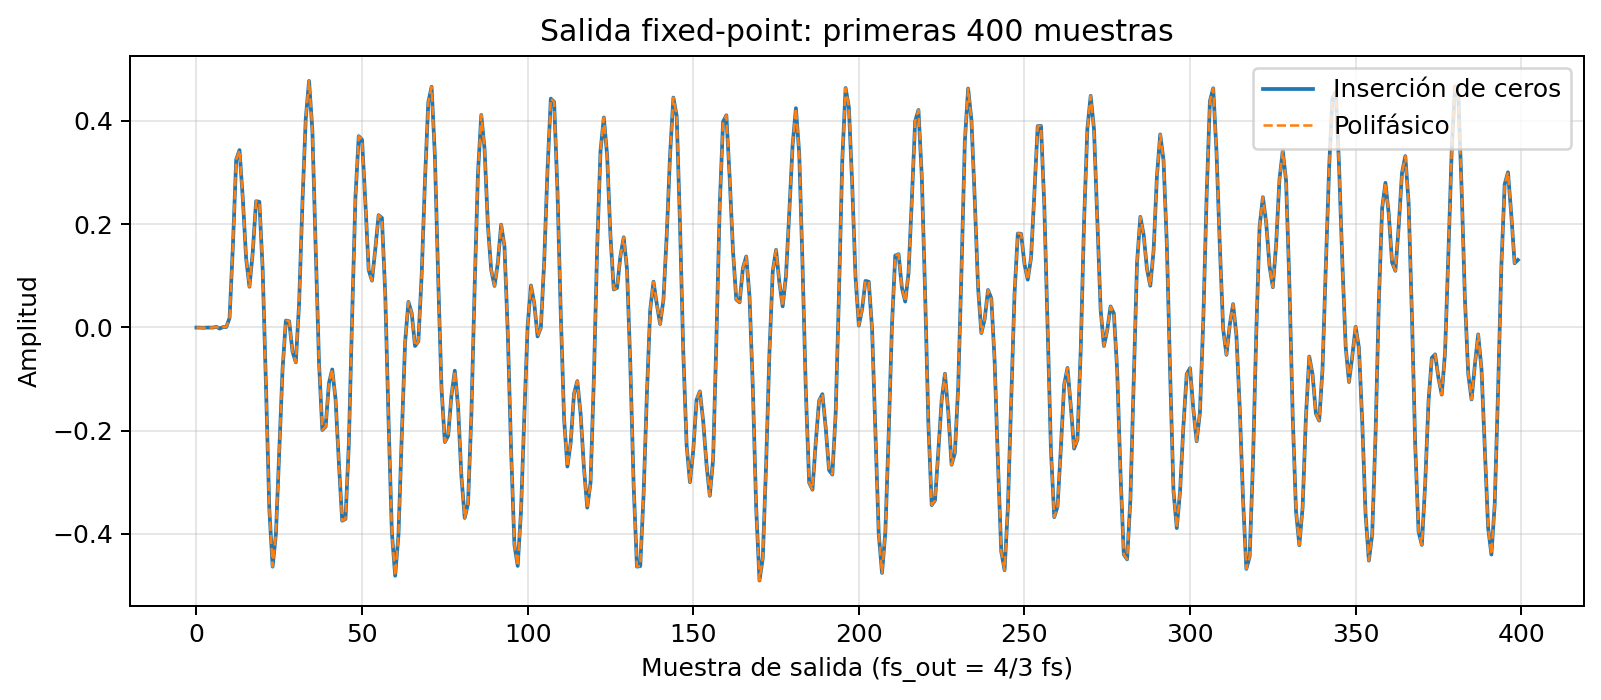
\includegraphics[width=0.88\linewidth]{interpolator_output.png}
    \caption{Salida de punto fijo del remuestreador $4/3$.}
    \label{fig:interpolator-output}
\end{figure}

\begin{figure}[H]
    \centering
    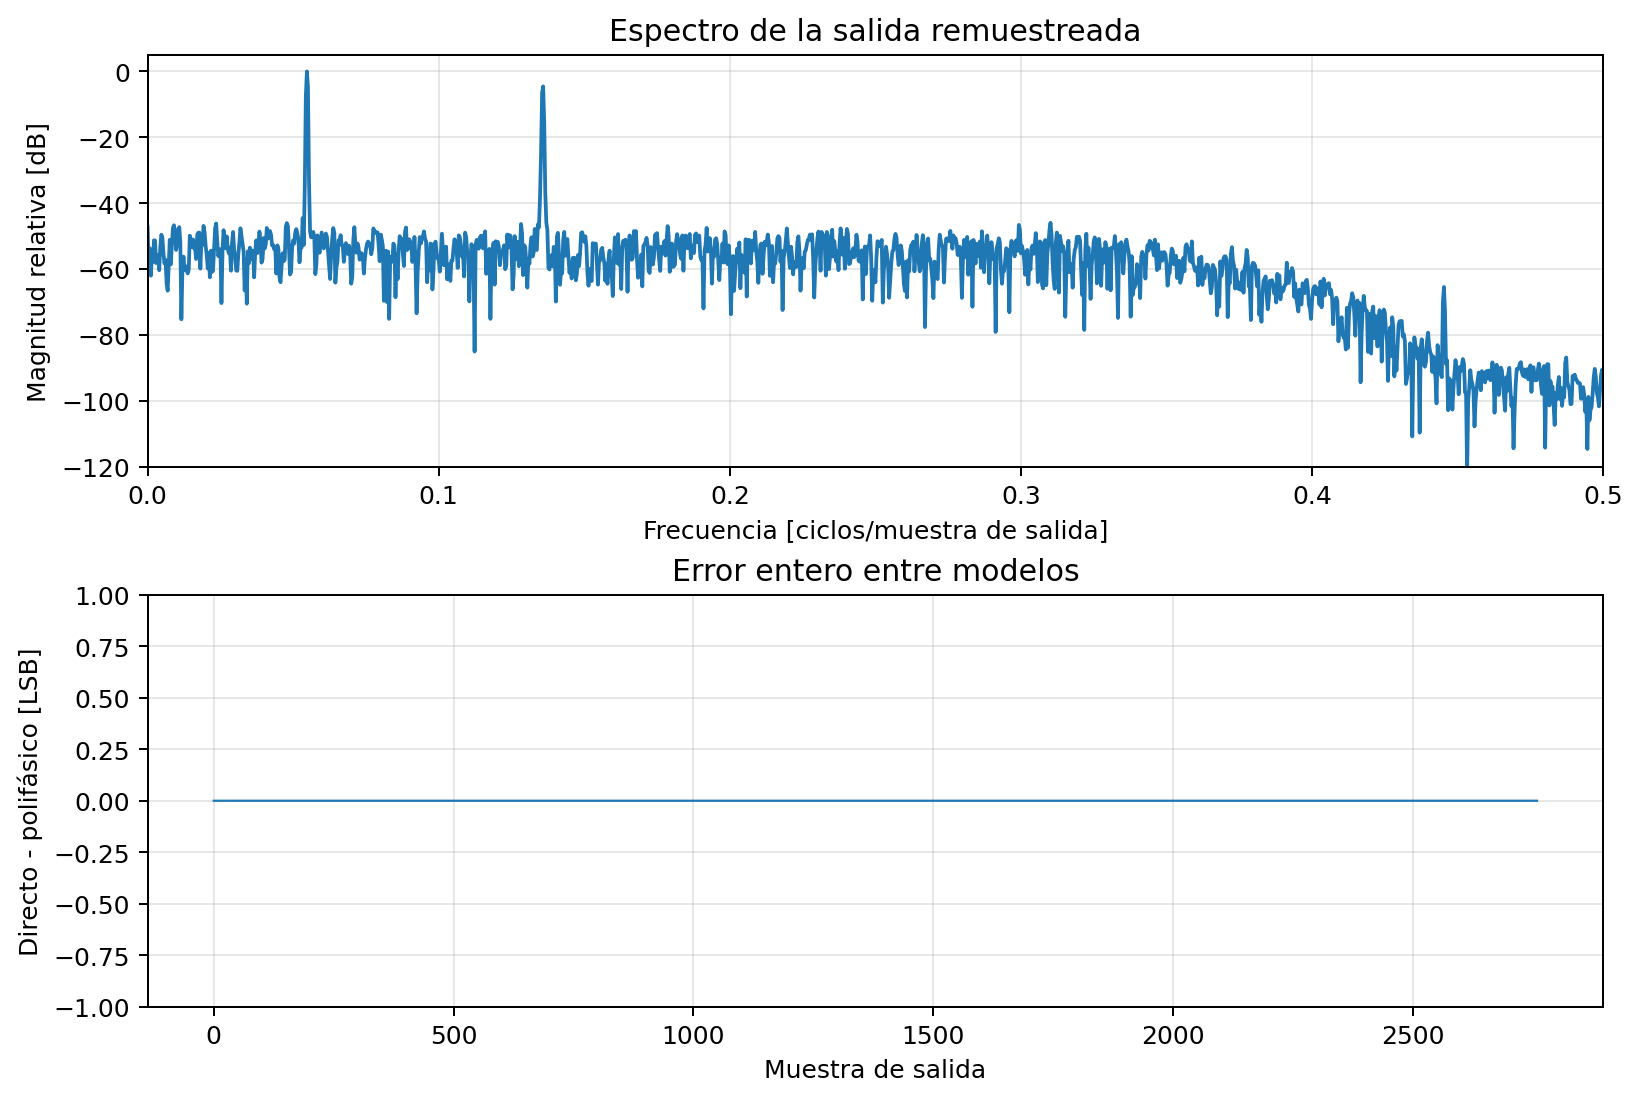
\includegraphics[width=0.88\linewidth]{output_spectrum_and_error.png}
    \caption{Espectro de salida y error muestra a muestra entre los dos modelos.}
    \label{fig:output-spectrum-error}
\end{figure}

% ---------------------------------------------------------------------------
\subsection{Implementaciones RTL}
\label{sec:rtl}
% ---------------------------------------------------------------------------

\subsubsection*{Interfaz común}

Las dos arquitecturas exponen la misma interfaz. El único clock trabaja a la tasa
$L f_s$ y \texttt{i\_valid} indica la llegada de una muestra nueva a $f_s$, por lo
que permanece alto un ciclo de cada cuatro. Después de completar la latencia
inicial, \texttt{o\_valid} acompaña una muestra de salida en todos los ciclos.

La interfaz RTL común se declara de la siguiente forma. En
\texttt{interp\_poly} solamente cambian el nombre del módulo y el paquete propio
importado; la lista de puertos es idéntica.

\begin{lstlisting}[language=Verilog,caption={Interfaz RTL común de los interpoladores.},label={lst:interfaz}]
module interp
    import interp_pkg::*;
    import fir_pkg::*;
(
    input  logic  i_clk,    // Clock a L*f_s
    input  logic  i_rst,    // Reset asincronico activo en alto
    input  logic  i_valid,  // Muestra nueva, un ciclo de cada L
    input  data_t i_data,   // Muestra signed Q1.11

    output logic  o_valid,  // Indica una salida valida
    output data_t o_data    // Resultado signed Q1.11
);
\end{lstlisting}

\subsubsection*{FIR compartido}

Ambas implementaciones reutilizan el mismo módulo \texttt{fir.sv} ya que, a fin 
de cuentas, se trata conceptualmente del mismo filtro. Sin embargo, cada variante
posee un paquete propio que determina la cantidad de taps y, por lo tanto, los
tipos de los buses internos y el ancho del acumulador. En el modulo FIR se encuentra 
el shift register, los productos parciales, la suma con precisión completa y el 
bloque común de truncamiento y saturación.

En la implementación directa el paquete configura 16 taps. En la polifásica se
utilizan cuatro instancias del mismo RTL, cada una configurada con 4 taps y
con los coeficientes de una fase diferente.

\figpendiente{Insertar captura del esquemático RTL de \texttt{fir}.}
{Arquitectura RTL del filtro FIR genérico.}

\subsubsection*{Interpolador mediante inserción de ceros}

La arquitectura \texttt{interp\_zeros} sustituye \texttt{i\_data} por cero durante
los ciclos en los que \texttt{i\_valid} está inactivo. El FIR permanece habilitado
en todos los ciclos y, por lo tanto, su línea de retardo contiene explícitamente
los tres ceros insertados entre muestras consecutivas.

La primera entrada válida se incorpora a la línea de retardo en el ciclo en el que
se recibe. El registro de salida del FIR captura el primer resultado en el ciclo
siguiente, por lo que la latencia de la arquitectura es de un ciclo del clock de
alta tasa. A partir de ese momento se produce una salida válida por ciclo.

\figpendiente{Insertar captura del esquemático RTL de \texttt{interp\_zeros}.}
{Arquitectura RTL del interpolador mediante inserción de ceros.}

\subsubsection*{Interpolador polifásico}

La arquitectura \texttt{interp\_poly} instancia cuatro FIR de cuatro taps. Todos
reciben la misma muestra de entrada y avanzan simultáneamente cuando
\texttt{i\_valid} está activo. Como este pulso aparece una vez cada cuatro ciclos,
cada subfiltro trabaja efectivamente a la tasa $f_s$. Sus salidas registradas se
entregan mediante un selector que recorre las fases 0, 1, 2 y 3.

El FIR actualiza el resultado correspondiente a una muestra en el siguiente evento
de habilitación. Como estos eventos están separados por cuatro clocks, la primera
salida de la arquitectura polifásica aparece cuatro ciclos después de aceptar la
primera entrada. Luego el selector entrega una salida por ciclo sin interrupciones.

\figpendiente{Insertar captura del esquemático RTL de \texttt{interp\_poly}.}
{Arquitectura RTL del interpolador polifásico.}

\subsubsection*{Latencia y alineación}

La Tabla~\ref{tab:latencias} resume las latencias observadas desde el primer
\texttt{i\_valid}. La diferencia de tres ciclos no modifica la secuencia numérica y
se resuelve en la verificación utilizando \texttt{o\_valid}, sin introducir una
compensación específica para cada DUT.

\begin{table}[H]
    \centering
    \caption{Latencia de las implementaciones RTL actuales.}
    \label{tab:latencias}
    \begin{tabular}{@{}lcc@{}}
        \toprule
        \textbf{Arquitectura} & \textbf{Primera salida válida} & \textbf{Latencia} \\
        \midrule
        \texttt{interp\_zeros} & Ciclo 1 & 1 clock de $L f_s$ \\
        \texttt{interp\_poly}  & Ciclo 4 & 4 clocks de $L f_s$ \\
        \bottomrule
    \end{tabular}
\end{table}

\subsection{Conteo de multiplicaciones}

Ambas descripciones RTL contienen 16 multiplicadores, uno por tap en el FIR
directo y cuatro por cada una de las cuatro fases en el polifásico. Sin embargo, 
la diferencia está principalmente en la tasa de productos, el FIR directo hace 
16 productos por cada salida a $L f_s$, aunque solamente cuatro operandos de 
datos son distintos de cero. La arquitectura polifásica hace 16 productos en 
paralelo una vez cada 4 ciclos, equivalentes a 4 productos por cada salida a 
$L f_s$.

\begin{table}[H]
    \centering
    \caption{Conteo estructural y actividad aritmética.}
    \label{tab:multiplicaciones}
    \begin{tabular}{@{}lccc@{}}
        \toprule
        \textbf{Arquitectura} & \textbf{Multiplicadores RTL} &
        \textbf{Productos por salida} & \textbf{Tasa de productos} \\
        \midrule
        Inserción de ceros & 16 & 16 & $16L f_s=64f_s$ \\
        Polifásica         & 16 & 4  & $4L f_s=16f_s$ \\
        \bottomrule
    \end{tabular}
\end{table}

Por lo tanto, la arquitectura polifásica reduce en un factor $L=4$ la cantidad de
operaciones por unidad de tiempo. Este es un conteo de la descripción RTL; la
implementación final de los productos con coeficientes constantes se verificará en
los reportes de síntesis.

% ---------------------------------------------------------------------------
\subsection{Verificación RTL}
\label{sec:verificacion-rtl}
% ---------------------------------------------------------------------------

\subsubsection*{Entorno de verificación común}

Se adaptó un entorno basado en clases compuesto por generador, driver, monitor y
scoreboard. El mismo testbench se utiliza para ambas arquitecturas; solamente cambia
el módulo seleccionado durante la compilación.

El generador lee las 2000 entradas cuantizadas exportadas por el modelo de Python.
Cada muestra se aplica con \texttt{i\_valid} activo durante un ciclo y se insertan
tres ciclos inactivos antes de la muestra siguiente. Al finalizar se envían muestras
nulas adicionales, manteniendo el mismo protocolo, para vaciar las líneas de retardo.

El monitor ignora la latencia particular del DUT y publica una muestra únicamente
cuando \texttt{o\_valid} está activo. El scoreboard lee las 8015 palabras del archivo
golden y las compara, informando frente a una eventual diferencia.

\subsubsection*{Resultados}

La simulación RTL de ambas implementaciones finalizó correctamente. Para cada DUT,
el scoreboard comparó las 8015 muestras válidas contra el mismo archivo de referencia
y no detectó diferencias. De esta forma se confirmó la equivalencia bit a bit entre
\texttt{interp\_zeros}, \texttt{interp\_poly} y el modelo fixed-point de Python.

La comparación comienza con la primera activación de \texttt{o\_valid}; por lo tanto,
la diferencia de tres ciclos entre las latencias de los DUT no requiere modificar el
estímulo ni mantener dos secuencias esperadas.

\figpendiente{Insertar captura de ondas con \texttt{i\_valid}, \texttt{i\_data},
\texttt{o\_valid} y \texttt{o\_data}; idealmente mostrar el inicio de ambas
simulaciones para evidenciar sus latencias.}
{Inicio de la simulación RTL y primera salida válida de cada arquitectura.}

% ---------------------------------------------------------------------------
\subsection{Barrido de síntesis y frecuencia máxima}
\label{sec:barrido-timing}

Se sintetizó cada arquitectura con períodos de clock decrecientes a partir de 1ns. 
La Tabla~\ref{tab:barrido-timing} resume los reportes del escenario  \texttt{func\_slow}. 
Se presentan el WNS y el TNS, junto con la cantidad de caminos en violación de setup.

\begin{table}[H]
    \centering
    \caption{Barrido de síntesis.}
    \label{tab:barrido-timing}
    \small
    \begin{tabular}{@{}lrrrrrr@{}}
        \toprule
        \textbf{Arquitectura} & $f$ [GHz] & $T$ [ns] &
        WNS [ns] & TNS [ns] & $n_{\mathrm{path}}$ \\
        \midrule
        Inserción de ceros & 1  & 1.000 & $0.00$  & $0.00$  & 0 \\
                          & 2   & 0.500 & $0.00$  & $0.00$  & 0 \\
                          & 2.5 & 0.400 & $-0.00$ & $-0.00$ & 1 \\
                          & 3   & 0.333 & $-0.00$ & $-0.00$ & 1 \\
                          & 4   & 0.250 & $-0.00$ & $-0.00$ & 4 \\
        \midrule
        Polifásica        & 1   & 1.000 & $0.00$  & $0.00$  & 0 \\
                          & 2   & 0.500 & $0.00$  & $0.00$  & 0 \\
                          & 3   & 0.333 & $0.00$  & $0.00$  & 0 \\
                          & 3.5 & 0.285 & $-0.00$ & $-0.00$ & 3 \\
                          & 4   & 0.250 & $-0.00$ & $-0.00$ & 7 \\
        \bottomrule
    \end{tabular}
\end{table}

Según los resultados obtenidos en los reportes del barrido de sintesis, las frecuencias
máximas sin violaciones de timing para cada arquitectura son:

\begin{equation}
f_{\max,\mathrm{zeros}}\approx 2.5\,\mathrm{GHz},
\qquad
f_{\max,\mathrm{poly}}\approx 3\,\mathrm{GHz}.
\label{eq:fmax-aproximadas}
\end{equation}

\subsubsection*{Caminos críticos}

En \texttt{interp\_zeros}, el recorrido crítico predominante parte de un registro
de la línea de retardos del FIR, atraviesa la lógica aritmética de los productos
por coeficientes constantes, el arbol de sumas y termina en el registro de salida
del FIR. En el reporte, el punto de partida exacto es \path{u_fir/data_r_reg} y
el de llegada \path{u_fir/o_data_reg}.

En \texttt{interp\_poly}, el camino crítico es el que conecta los registros
de muestras con los registros de resultado de las fases. En el reporte,
parte de \path{gen_phases.u_fir_phase/data_r_reg} y termina en
\path{gen_phases.u_fir_phase/o_data_reg}. La división en subfiltros de cuatro 
taps reduce la profundidad del arbol de sumas respecto del FIR directo de 16 
taps. Esto permite alcanzar una frecuencia máxima mayor en el barrido realizado.


\subsection{Frecuencia y período de trabajo comunes}
\label{sec:periodo-comun}

Se fija como frecuencia de trabajo en común la $f_{\mathrm{clk}}=2\,\mathrm{GHz}$,
ya que deja un margen de aproximadamente 20\,\% respecto a la máxima frecuencia 
para la cual la arquitectura directa cierra timing. Este margen se deja para 
conservar espacio para las modificaciones posteriores y, al mismo tiempo, evitar 
una síntesis  casi exclusivamente HVT como la observada a 1 GHz.

La Tabla~\ref{tab:vt-trabajo} muestra que a 2 GHz ambas síntesis utilizan los cuatro
tipos de celdas. Los porcentajes corresponden a cantidad de celdas, según
\texttt{vt\_groups.rpt}.

\begin{table}[H]
    \centering
    \caption{Distribución de celdas por tensión de umbral a la frecuencia común de 2 GHz.}
    \label{tab:vt-trabajo}
    \begin{tabular}{@{}lrrrr@{}}
        \toprule
        \textbf{Arquitectura} & HVT [\%] & RVT [\%] & LVT [\%] & SLVT [\%] \\
        \midrule
        Inserción de ceros & 69.80 & 1.41 & 20.08 & 8.71 \\
        Polifásica        & 73.60 & 0.79 & 20.22 & 5.40 \\
        \bottomrule
    \end{tabular}
\end{table}

La presencia de celdas LVT y SLVT deja una oportunidad para estudiar el compromiso
entre leakage y timing mediante multi-$V_t$ en el Ejercicio 6.

% ---------------------------------------------------------------------------
\subsection{Simulación a nivel de compuertas (GLS)}
\label{sec:gls}

En esta etapa se ejecutó la simulación a nivel de compuertas sobre ambas 
arquitecturas con los retardos SDF anotados. En un primer momento, al ejecutar
\texttt{make gls}, aparecieron las violaciones de ancho de pulso \texttt{\$width} 
advertidas en la consigna, asociadas a los límites genéricos de los modelos de 
librería.  Por ejemplo, en registros del FIR directo se informó un límite de 
1000 ps frente a intervalos de 250 ps. A la frecuencia de trabajo de 2 GHz, 
el período es de 500 ps y el semiperíodo nominal es de 250 ps, por lo que ese 
límite de 1 ns se incumple aun con el clock previsto para el diseño.

Estos mensajes se identificaron como falsas violaciones debidas al placeholder
de ancho de pulso del modelo, por lo que no corresponden a violaciones de setup o
hold del camino de datos.

Luego se ejecutó \texttt{make gls-ntc}, que deshabilita los chequeos de timing
mediante \texttt{+notimingcheck} y conserva los retardos SDF. Ambas arquitecturas
completaron correctamente la simulación y la comparación bit a bit con el modelo
de referencia. Estas corridas se utilizaron para obtener la actividad de potencia.

% ---------------------------------------------------------------------------
\subsection{Estimación de potencia con actividad de GLS}
\label{sec:potencia-inicial}

En esta etapa, se convirtió a SAIF la actividad obtenida de GLS con SDF y
se ejecutó PrimeTime PX en modo de potencia promedio. La comparación utiliza el
mismo estímulo y una frecuencia común de 2 GHz. El reporte de actividad confirmó
una cobertura de anotación del 100\,\% en ambas arquitecturas.

\begin{table}[H]
    \centering
    \caption{Potencia estimada con PrimeTime PX a 2 GHz y actividad de GLS con SDF.}
    \label{tab:potencia-inicial}
    \begin{tabular}{@{}lrrr@{}}
        \toprule
        \textbf{Magnitud} & \textbf{Inserción de ceros} & \textbf{Polifásica} &
        \textbf{Reducción [\%]} \\
        \midrule
        Switching [mW]          & 4.516  & 2.351  & 47.9 \\
        Internal [mW]           & 1.964  & 0.5207 & 73.5 \\
        Leakage [$\mu$W]        & 17.68  & 14.24  & 19.5 \\
        Potencia total [mW]     & 6.497  & 2.886  & 55.6 \\
        Energía por salida [pJ] & 3.249  & 1.443  & 55.6 \\
        \bottomrule
    \end{tabular}
\end{table}

La energía por muestra se calculó dividiendo la potencia total por la tasa de
salida, que coincide con la frecuencia de clock de 2 GHz. La arquitectura
polifásica reduce la potencia total un 55.6\,\%, con una relación

\begin{equation}
\frac{P_{\mathrm{zeros}}}{P_{\mathrm{poly}}}
=
\frac{6.497}{2.886}
\approx 2.25.
\label{eq:relacion-potencias}
\end{equation}

Este factor es menor que el ahorro aritmético teórico $L=4$, ya que la potencia
total también incluye el consumo de registros y de la distribución de clock.
Además, la arquitectura polifásica incorpora lógica de selección y control de
fases, cuyos consumos no escalan proporcionalmente con la cantidad de productos
por muestra. La reducción relativa más marcada se observa en la potencia interna,
del 73.5\,\%, mientras que la potencia de switching disminuye un 47.9\,\%. El
leakage se reduce un 19.5\,\% y representa menos del 0.5\,\% de la potencia total
en ambas variantes; por lo tanto, en estas condiciones domina la potencia dinámica.

\begin{table}[H]
    \centering
    \caption{Desglose de potencia total por grupo a 2 GHz.}
    \label{tab:potencia-grupos-inicial}
    \begin{tabular}{@{}lrrr@{}}
        \toprule
        \textbf{Grupo} & \textbf{Zeros [mW]} & \textbf{Poly [mW]} &
        \textbf{Cambio [\%]} \\
        \midrule
        Combinacional & 4.993  & 1.576  & $-68.4$ \\
        Registros     & 0.8891 & 0.5678 & $-36.1$ \\
        Red de clock  & 0.6148 & 0.7418 & $+20.7$ \\
        \bottomrule
    \end{tabular}
\end{table}

En base al desglose de potencia por grupos, se puede observar que la lógica
combinacional concentra el 76.85\,\% del consumo de \textit{zeros} y el
54.61\,\% del de \textit{poly}. Su reducción de aproximadamente 3.417 mW explica
la mayor parte del ahorro absoluto. Esto evidencia que la arquitectura polifásica
genera un ahorro considerable al calcular únicamente los productos que
efectivamente contribuyen a cada muestra de salida.

Los registros también consumen menos en la arquitectura polifásica, aunque su
reducción es menor. En cambio, la red de clock aumenta un 20.7\,\% en potencia
absoluta y pasa de representar el 9.46\,\% al 25.71\,\% del total. Este incremento
se debe a que la reorganización del procesamiento en fases modifica la estructura
secuencial del circuito y aumenta la carga efectiva asociada al clock, aun cuando
la lógica combinacional total se reduzca.

\end{document}
